\documentclass{beamer}
\usepackage[english]{babel}
\usepackage[utf8]{inputenc}
\usepackage{xcolor}
\usepackage{beamerthemesplit}
\usepackage[orientation=landscape, size=custom, width=16, height=9, scale=0.5]{beamerposter}
\usetheme[left]{AAUsidebar}

\title{Privacy methods.}
\subtitle{Simulazione di Sistemi}
\date{\today}

\author[Davide Berardi, Matteo Martelli]{
	Davide Berardi
	\and
	Matteo Martelli
	\\
	0000712698
	\and
	0000702472
}

\institute[Simulazione di Sistemi]{Università di Bologna.}


\begin{document}
\pgfdeclareimage[height=1.7cm,width=1.7cm]{titlepagelogo}{AAUgraphics/Lock}

\titlegraphic{
	\pgfuseimage{titlepagelogo}
}
{
	\aauwavesbg
	\begin{frame}[plain,noframenumbering]
		\titlepage
	\end{frame}
}

%\begin{frame}{Table of contents}{}
	%\tableofcontents
%\end{frame}

% Parte 1
\section{Introduction}

\begin{frame}
	\frametitle {Privacy}
	Privacy is the right to publish only some informations that we want to
	publish.\\

	There are a lot of laws and legal issues related to privacy (but some
	people are just not interested in laws).
\end{frame}

\begin{frame}
	\frametitle {Anonymity}
	We will talk about anonymity as the propriety of disconnect the user of a
	service from some basic proprieties:
	\begin{itemize}
		\item Geolocation.
		\item Association to a face or a name (or to an IP address).
	\end{itemize}

	Sometimes we need to re-associate the user with a communication
	channel or so.
\end{frame}

\section{Who's involved?}
%"I have nothing to hide, who cares about my personal data?"
\begin{frame}
	\frametitle{But...who cares?}
\end{frame}

\subsection{Surveillance} 
%I would start with the big picture of the Utah Datacenter
%NSA, snowden leaks
\begin{frame}
	\frametitle{Surveillance}
\end{frame}

\begin{frame}
	\frametitle{NSA projects}
\end{frame}

\begin{frame}
	\frametitle{Other stories}

	% Zimmermann
	% Lavabit
	% IP-sec (6)
	% Truecrypt
\end{frame}

\subsection{Obscuring}
%china, mid-east
\begin{frame}
	\frametitle{Obscuration}
	% Geo-obscuring
	% SOPA and PIPA
\end{frame}

\subsection{Companies} %? needed ?
%focused adv, industrial espionage
\begin{frame}
	\frametitle{Industrial espionage}
\end{frame}

\subsection{Bad Guys}
%(identity stealing, money stealing, etc.)
\begin{frame}
	\frametitle{Not only powerful adversaries}
\end{frame}
 %gov (surveillance, obscuring), bad_guys
\section{Programs}
\begin{frame}
	\frametitle{Technologies}
	What we can do versus controls?\\
	Can we have some privacy even from the companies/government?
\end{frame}

\begin{frame}
	\frametitle{Confidentiality and authenticity}
	We have a lot of programs to protect our data
	\begin{itemize}
		\item PGP
		\item IPsec
		\item OTR-based programs
		\item Protonmail 
\includegraphics[scale=0.017]{imgs/Protonmail_logo}
		\item TrueCrypt 
\includegraphics[scale=0.1]{imgs/TrueCrypt_Logo}
		\item \textbf{Perfect Forward Secrecy}
	\end{itemize}
	Some tool for steganography can help but not too much.
\end{frame}

\begin{frame}
	\frametitle{Anonymity}
	But for anonymity?
	\begin{itemize}
		\item Anonymous networks
		\item Mix Max networks.
		\item Anonymous remailers.
		\item Proxy chains.
		\item \textbf{Onion Routers}
	\end{itemize}
\end{frame}

\begin{frame}
	\frametitle{Anonymous network}
	(mostly) p2p-based networks, no one can identify who put a file on the
	net.
	\begin{itemize}
		\item FreeNet 
\includegraphics[scale=.5]{imgs/Freenet_logo}
		\begin{itemize}
			\item OpenNet mode
			\item DarkNet mode
		\end{itemize}
		\item GNUNet \includegraphics[scale=0.1]{imgs/GNUnet_logo}
	\end{itemize}

	\begin{itemize}
		\item Fully Self Contained (like UseNet).
		\item Search?
		\item Performance?
	\end{itemize}
\end{frame}

\begin{frame}
	\frametitle{Mix Networks}
	\begin{minipage}{0.49\textwidth}
	\begin{itemize}
		\item Model of the 1981.
		\item Multiple layers of encryption.
		\item Select different random nodes to deal with controlled
		nodes.
		\item \textbf{Timing attack?}
	\end{itemize}
	\end{minipage}
	\begin{minipage}{0.5\textwidth}
	\begin{center}
		
\includegraphics[width=0.7\textwidth]{imgs/mix_networks.png}\\
		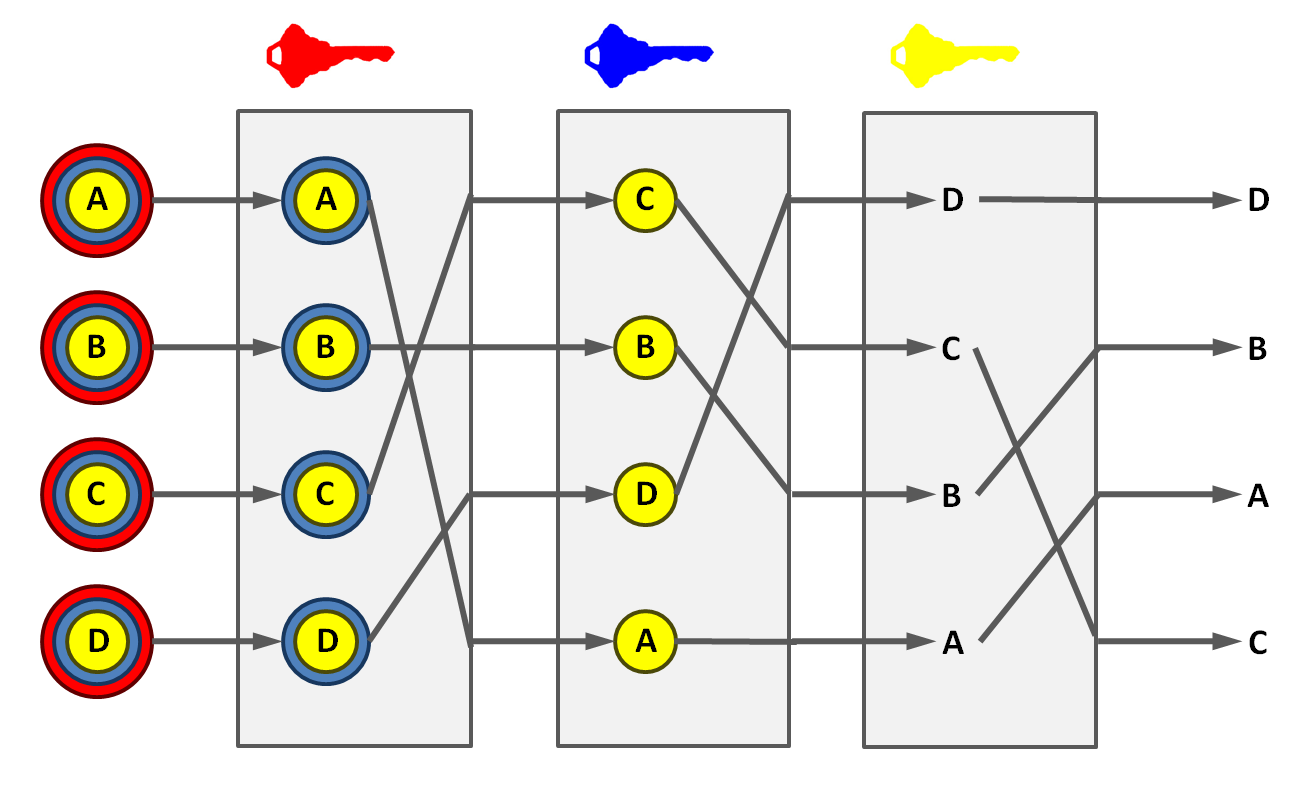
\includegraphics[width=0.7\textwidth]{imgs/Decryption_mix_net.png}
	\end{center}
	\end{minipage}
\end{frame}

\begin{frame}
	\frametitle{Old times}
	\begin{itemize}
		\item Anonymous remailers: end to end anonymity.
		\begin{itemize}
			\item Cypherpunk: remove FROM field and encrypt the mail
			\item Mixmaster: Chain of remailers.
			\item Mixminion: Mixmaster syntax with replies.
			\item nym-server: give a pseudonym to the user detached
			from his IP.
		\end{itemize}
		We'll see that this servers recalls the modern idea of
		OnionRouting.
	\end{itemize}
\end{frame}

\begin{frame}
	\frametitle{Onion Routing}
	The idea of encapsulate cyphered packets in a chain or an "onion".

	\begin{itemize}
		\item OpenNet? $\to$ Hidden services.
		\item New possibility like use a proxy to get to the normal
		internet.
	\end{itemize}
	\begin{block}{Problems}
	\begin{itemize}
		\item Performance
		\item DoS resistance.
		\item Mantain links to the users
		\item Thrustness of the routers.
		\item Confidentiality and autenticity.
	\end{itemize}
	\end{block}
\end{frame}

\begin{frame}
	\frametitle{Onion Routing (2)}

	\begin{itemize}
		\item TOR 
\includegraphics[scale=0.1]{imgs/Tor_logo}
		\begin{itemize}
			\item We'll come to this later.
		\end{itemize}
		\item i2p 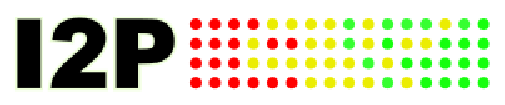
\includegraphics[scale=0.2]{imgs/I2P_logo}
		\begin{itemize}
			\item Done for eepsite(s).
			\item Not so much routers/outproxies.
		\end{itemize}
	\end{itemize}
	\begin{itemize}
		\item And what for the low latency? $\to$ \textbf{Timing attacks}.
	\end{itemize}
\end{frame}

\begin{frame}
	\frametitle{Why simulation?}
	Simulation help us in a lot of aspects:

	\begin{itemize}
		\item Compare the performances of two onion routers (p.e. i2p vs
		Tor).
		\item To compare effects of changes in the node choice
		algorithms.
		\item \textbf{Get an idea of the number of resources needed by an
		attacker and to mantain anonimity}.
	\end{itemize}
\end{frame}

\section{Tor}
\begin{frame}
	\frametitle{NSA and Tor}
	Tor was made from the naval research labs:
	\begin{itemize}
		\item Made for the anonymous control and espionage.
		\item Tor need a number of exit nodes (and routers) to lead
		anonymity to an user.
		\item if an organization use only his exit nodes it's like to
		not use them at all.
	\end{itemize}
\end{frame}

\begin{frame}
	\frametitle{The Tor revolution}
	Apparently Tor slipped from the hands of the US in the 2004.
	\begin{minipage}{.49\textwidth}

	\begin{itemize}
		\item Russia offered \$114.000 to identify and deface Tor
		anonimity.
		\item NSA now classify TOR as a menace of level
		\textit{catastrophic}.
	\end{itemize}
	\end{minipage}
	\begin{minipage}{.5\textwidth}
		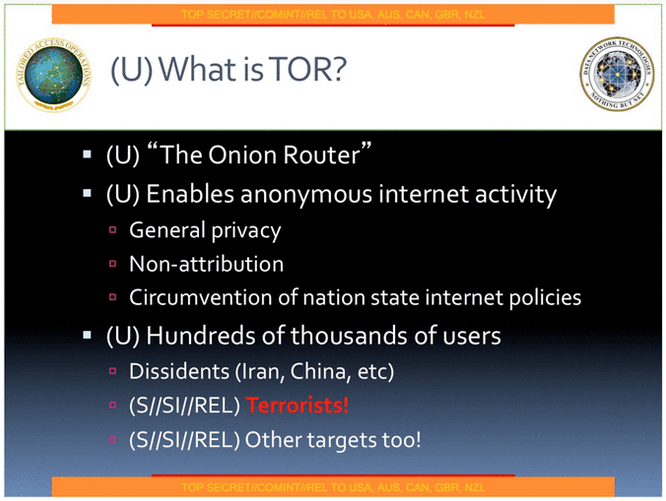
\includegraphics[scale=0.35]{imgs/nsa_tor}
	\end{minipage}
	But...nobody knows who and what is hidden under the layer of the onion.
\end{frame}


% Parte 2
%Tor internal working
 %working (briefly)

\section{Timing Attack}
\begin{frame}{Time analysis based attacks}{}
	\begin{quote}
		\emph{``Tor does not provide protection against end-to-end timing attacks[...]''}
	\end{quote}
	We can place a tracker after the client node and another before the server node
	and check for the connection time to profile users and nodes (and later associate IP to users.)
\end{frame}


%attacks, timing, our project -> NSA ueses timing
 %attacks, timing, our project, NSA timing
\section{Astoria}
\begin{frame}{Measuring AS-level adversaries against Tor}
	\begin{itemize}
		\item Multiple Autonomous Systems (AS) collude with each other
	performing time based attacks and collecting asymmetric data.

		\item Up to 40\% of circuits constructed by the current Tor
	client are vulnerable to AS-level attackers.

		\item Connections  from  China  were  found  to  be  most  vulnerable 
	to AS-level attackers with up to 86\% of
	all  Tor  circuits.
	\end{itemize}
\end{frame}


\begin{frame}{Mitigating AS-level adversaries against Tor}{ASes
correlations}

	Connections between ASes are negotiated as business arrangements.
\begin{figure}
			\centering
			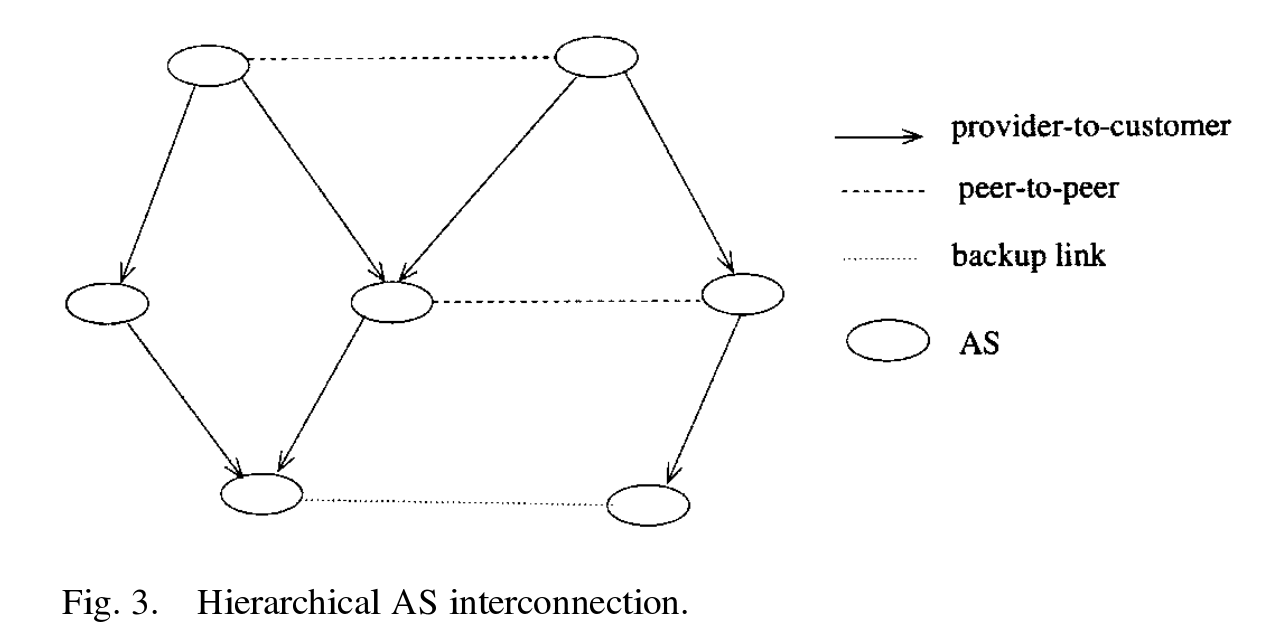
\includegraphics[scale=0.18]{imgs/as_graph.png}
		\end{figure}

	\begin{block}{The idea}
		Building a graph of ASes correlations to identify vulnerable
	paths.
	
	\end{block}
\end{frame}

\begin{frame}{Astoria}

	\begin{itemize}
		\item Use of path prediction to avoid Tor vulnerable paths.\\
	i.e. The entry node and the exit node may be selected together if their ASes 
	are unrelated to each others.
		\item Able to perform  load-balancing at least as well as the vanilla Tor
client.
	\end{itemize}

\end{frame}


%\section{Other ORs and technologies}
%\subsection{HORNET}
	%change OR model
	%faster because does not encrypt the payload for each relay (only
	%the headers)
	%protects also against timing attacks?

\section{Possible Solutions}
\begin{frame}{Possible Solutions}
	User awareness on privacy and anonymity.
	\begin{figure}
		\centering
		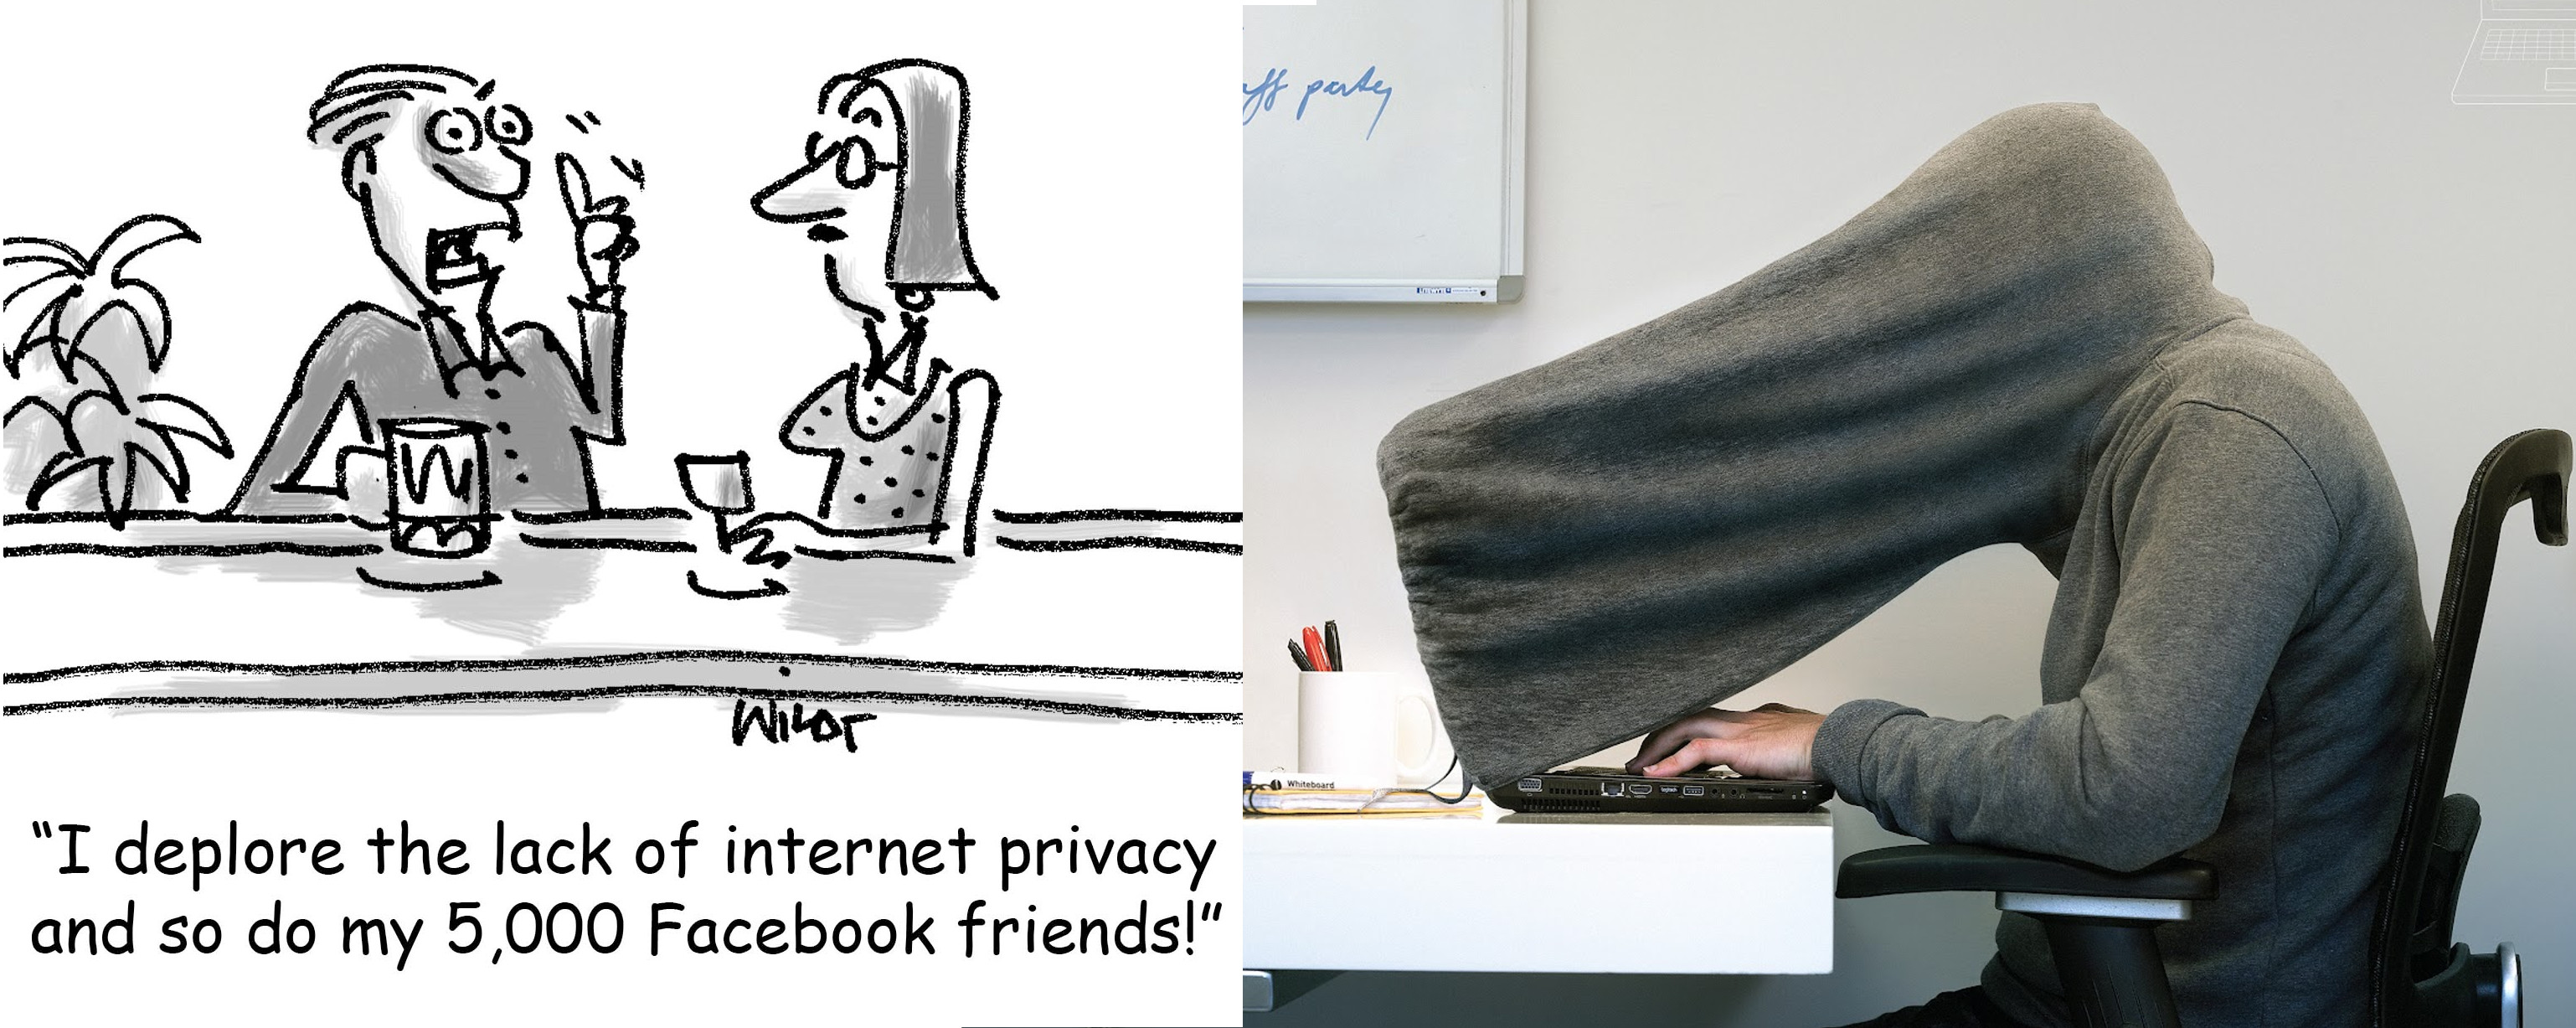
\includegraphics[scale=0.50]{imgs/user_privacy.jpg}
	\end{figure}
\end{frame}

\begin{frame}{Possible Solutions}
	\begin{itemize}
		\item Need of privacy rules reinforcement and more investments on network
security solutions\\
			\small{(i.e. In April 2014, the European Court of Justice declared
invalid the EU Data Retention Directive.)\footnote{According to the directive, 
member states will have to store citizens' telecommunications data for a minimum 
of 6 months and at most 24 months. Under the directive the police and security 
agencies will be able to request access to details such as IP address and time 
of use of every email, phone call and text message sent or received.}}
		\item Academic researches
		\item FOSS
	\end{itemize}	
\end{frame}

 %other ORs, astoria, IPsec?

{
\aauwavesbg
\begin{frame}[plain,noframenumbering]
	\finalpage{Thank you for your attention.}
\end{frame}
}

\end{document}
